\documentclass{article}
\setlength{\parskip}{5pt} % esp. entre parrafos
\setlength{\parindent}{0pt} % esp. al inicio de un parrafo
\usepackage{amsmath} % mates
\usepackage[sort&compress,numbers]{natbib} % referencias
\usepackage{url} % que las URLs se vean lindos
\usepackage[top=25mm,left=20mm,right=20mm,bottom=25mm]{geometry} % margenes
\usepackage{hyperref} % ligas de URLs
\usepackage{graphicx} % poner figuras
\usepackage[spanish]{babel} % otros idiomas
\usepackage[utf8]{inputenc} % alparecer son los acentos
\documentclass[12pt,letterpaper]{article}
\usepackage[utf8]{inputenc}
\usepackage{tikz}
\usetikzlibrary{trees}
\usepackage[spanish, es-nodecimaldot]{babel}
\usepackage{color}
\usepackage{algorithm}
\usepackage[noend]{algpseudocode}
\renewcommand{\algorithmicrequire}{\textbf{Entrada:}}
\renewcommand{\algorithmicensure}{\textbf{Salida:}}
\usepackage{subcaption}
\usepackage{amsfonts}
\usepackage{hyperref}
 \hypersetup{
     colorlinks=true,
     linkcolor=blue,
     filecolor=blue,
     citecolor = blue,      
     urlcolor=cyan,
     }
\usepackage{amssymb}
\usepackage{listings}
\usepackage{color}
\author{I E G} % author
\title{Práctica 5 : método Monte-Carlo} % titulo
\date{\today}

\begin{document} % inicia contenido

\maketitle % cabecera

\begin{abstract} % resumen
En esta práctica se usa el método Monte-Carlo que es idóneo para situaciones en las cuales algún valor o alguna distribución no es conocida en este caso tomaremos como ejemplo de que se conoce el valor de una integral \eqref{fx} y se calcula mediante el método Monte-Carlo como casa de estudio \cite{elis5} se trabaja estadísticamente la convergencia de la precisión del estimado del integral con el método Monte-Carlo comparando con el valor producido por Wolfram Alpha, en términos del número de decimales correctos, aumentando el tamaño de muestra.

\begin{equation} 
 \int_{3}^{7} f(x) dx 
\label{fx}
\
\end{equation}

\begin{equation}
f(x) = \frac{1}{exp(x) + exp(-x)}
\label{fx2}
\end{equation}
\smallskip

\end{abstract}


\section{Desarrollo}
Para efectos de esta práctica, se utiliza el paquete estadístico R versión 4.0.2 \cite{R}. Se pretende calcular el valor de la integral \eqref{fx}  para la función \eqref{fx2} empleando el método Monte-Carlo, y comparar el valor obtenido por Wolfram Alpha de 0.048834 \cite{wolf} para la generación del código previamente reportado en \cite{elis5} se utiliza también la herramienta de paralelización para que el código se ejecute con cuatro núcleos y realiza la generación de datos variando las muestras de $ 10^1 a 10^7$ con 150 réplicas, posteriormente grafica en diagramas caja-bigote.



  

\section{Experimento}


El programa ejecuta las operaciones para calcular un valor \cite{nat5} con cierto grado de precisión y lo compara con un valor de la referencia de Wolfram Alpha y verifica el numero de decimales coincididos para la precisión de el calculo obtenido de cada muestra, como se observa en la figura \ref{fig1} como incrementa el valor de los decimales coincididos demostrando que con mayor número muestras es más preciso el valor calculado.


\begin{figure} % figura
    \centering
    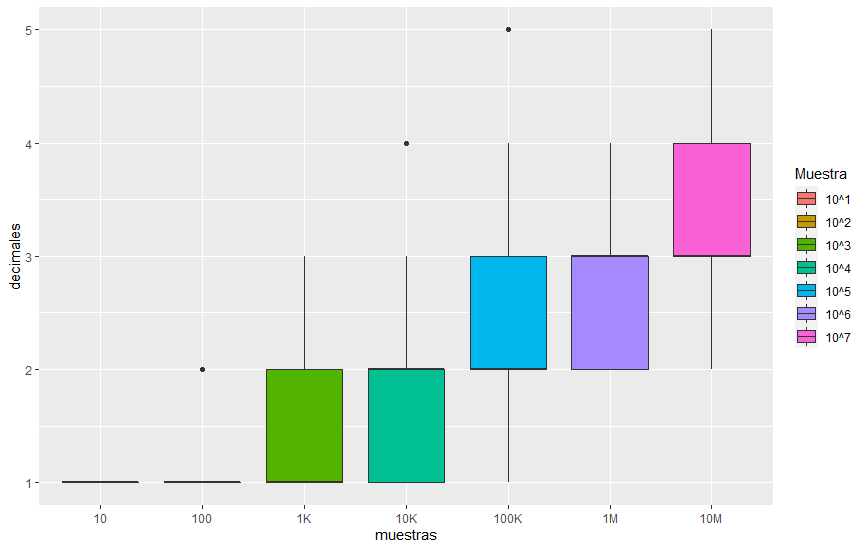
\includegraphics[width=170mm]{fig1.png} % archivo
    \caption{Diagramas de caja - bigote.}
    \label{fig1}
\end{figure}


 
\section{Conclusiones} 
En conclusión el método resulta muy útil para el cálculo con precisión de valores desconocidos y en aplicaciones varias de ingeniería. 



\bibliography{bib}
\bibliographystyle{plainnat}

\end{document}